% -*- tex -*-
%
\usepackage{ifthen}

\usepackage{tikz}
\usetikzlibrary{shapes,shadows,chains,shapes.multipart,arrows,positioning,fit}


\tikzstyle{inf} = [chamfered rectangle corners=north west, draw,text depth=.25ex]

\tikzstyle{lhs} = [signal, signal pointer angle=145,draw,signal to=nowhere,node
distance=0mm,text height=1.5ex,text depth=.25ex, signal from=east]

\tikzstyle{tgt} = [signal, signal pointer angle=145 , draw, signal to=nowhere,node distance=0mm,text height=1.5ex,text depth=.25ex, signal to=west,signal to=east,fill=gray!20]

\tikzstyle{rhs} = [signal, signal pointer angle=145 , draw, signal to=nowhere,node distance=0mm,text height=1.5ex,text depth=.25ex, signal from=west]

\tikzstyle{cls} = [rectangle, draw,node distance=0mm,text height=1.5ex,text depth=.25ex]
%different styles for cg, cd etc.^^

\tikzstyle{dist} = [rectangle,node distance=1mm,minimum size=6mm]

\begin{comment}
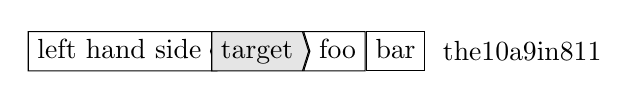
\begin{tikzpicture}
\node[lhs] (n0) {left hand side};
\node[tgt] (n1) [right=of n0] {target};
\node[rhs] (n2) [right=of n1] {foo};
\node[cls] (n3) [right=of n2] {bar};
\node[dist] (txt) [right=of n3] {\dist{the}{10}\dist{a}{9}\dist{in}{8}\dsum{1}{1}};
\end{tikzpicture}
\end{comment}



%wopr out: { W/M }{ CG/CD/IC }{ LHS }{ TARGET }{ RHS }{ CLASS }{ DISTR }
%            1       2          3      4         5       6       7
\newcommand{\wlr}[7]{\noindent\ensuremath{\begin{tikzpicture}
% first a place holder, haf the size of the WEX circle, so the
% WEX and  MONO boxes align.
\ifthenelse{\equal{#1}{w}}{
  \node (sp) [draw,fill=white,circle,inner sep=0pt,minimum size=0pt] {};
}{
  \node (sp) [draw=white,fill=white,circle,inner sep=0pt,minimum size=1.5pt] {};
}
% end if
\node[lhs] (n0) [right=of sp] {{\sf #3}};
% print dot if WEX (open dot if MONO, then we don't need (sp) ?)
\ifthenelse{\equal{#1}{w}}{
  \node (c1) at (n0.north west) [draw,fill,circle,inner sep=0pt,minimum size=3pt] {};
}{}
% end if
\node[tgt] (n1) [right=of n0] {{\sf #4}};
% RHS? If empty {}, skip, print rest
\ifthenelse{\equal{#5}{}}{
  \node[cls] (n3) [right=of n1] {{\sf #6}};
}{ % We do have a RHS
  \node[rhs] (n2) [right=of n1] {{\sf #5}};
  \node[cls] (n3) [right=of n2] {{\sf #6}};
} % end if RHS
% cross out if wrong answer
\ifthenelse{\equal{#2}{ic}}{
  \draw (n3.north east) -- (n3.south west);
}{}
% end if
% dotted if cd
\ifthenelse{\equal{#2}{cd}}{
  \draw [dotted, thick] (n3.north east) -- (n3.south west);
}{}
% end if
\node[dist] (txt) [right=of n3] {#7};
\end{tikzpicture}}}


% Instance
%
\newcommand{\tri}[3]{\makebox[1.5cm][l]{#1}\makebox[1.5cm][l]{#2}\makebox[1.5cm][l]{#3}}
\newcommand{\trit}[1]{\makebox[1.5cm][l]{#1}}
%
%instance l3
\newcommand{\ilt}[4]{\noindent\ensuremath{\begin{tikzpicture}
\node [rectangle, node distance=0mm,text height=1.5ex,text
depth=.25ex, draw] (i) {\tri{#1}{#2}{#3}};
\node [rectangle, node distance=0mm,text height=1.5ex,text depth=.25ex
, draw] (n1) [right=of i] {\trit{#4}};
\end{tikzpicture}}}
%
\newcommand{\bit}[1]{
\node [rectangle, node distance=0mm,text height=1.5ex,text depth=.25ex
, draw] {\bbx{#1}};
}
\newcommand{\OLDtrigram}[4]{\noindent\ensuremath{\begin{tikzpicture}
\bit{#1}\bit{#2}\bit{#3}\bit{#4}
\end{tikzpicture}}}
%
%%%
%
\newcommand{\bbx}[1]{\makebox[1.25cm][l]{\footnotesize{\sf #1}}}
\newcommand{\trigram}[4]{\noindent
\begin{tikzpicture}[start chain,node distance=1mm]
\node [on chain, drop shadow, rectangle, node distance=0mm,text height=1.5ex,text depth=.25ex
, draw, fill=white] {\bbx{#1}};
\node [on chain, drop shadow, rectangle, node distance=0mm,text height=1.5ex,text depth=.25ex
, draw, fill=white] {\bbx{#2}};
\node [on chain, drop shadow, rectangle, node distance=0mm,text height=1.5ex,text depth=.25ex
, draw, fill=white] {\bbx{#3}};
\node [on chain, drop shadow, rectangle, node distance=0mm,text height=1.5ex,text depth=.25ex
, draw, fill=gray!20] {\bbx{#4}};
\end{tikzpicture}
}

